% !TEX program = lualatex
% ============================================================
% つくばエクスプレス つくば駅における宇宙線測定装置の設置依頼書
% コンパイル: lualatex つくば駅_測定装置設置依頼書.tex
% ============================================================
\documentclass[a4paper,10pt]{ltjsarticle}

\usepackage{geometry}
\usepackage{booktabs}
\usepackage{array}
\usepackage{tabularx}
\usepackage{enumitem}
\usepackage{xcolor}
\usepackage{hyperref}
\usepackage{graphicx}
\usepackage{tikz}
\usetikzlibrary{arrows.meta,positioning}

\geometry{top=18mm, bottom=18mm, left=20mm, right=20mm}

\hypersetup{
  colorlinks=true,
  urlcolor=blue!50!black,
  pdfauthor={川嶋宥翔 / KEK Summer Challenge 2026 Team 9},
  pdftitle={つくば駅における宇宙線測定装置の設置に関するお願い},
}

\setlist[itemize]{leftmargin=1.5em, itemsep=0.1em, topsep=0.2em, parsep=0pt}
\setlist[enumerate]{leftmargin=1.5em, itemsep=0.1em, topsep=0.2em, parsep=0pt}
\setlength{\parindent}{1em}
\setlength{\parskip}{0.25em}

\newcommand{\DocDate}{2026年8月24日}
\newcommand{\ApplicantOrgA}{高エネルギー加速器研究機構（KEK）}
\newcommand{\ApplicantOrgB}{サマーチャレンジ 2026 演習9班}
\newcommand{\ApplicantName}{川嶋 宥翔}
\newcommand{\ApplicantAffiliation}{名古屋大学}
\newcommand{\ContactPhone}{080-8537-2616}
\newcommand{\ContactEmail}{kawashima.yuto.c2@s.mail.nagoya-u.ac.jp}
\newcommand{\AdvisorName}{岩瀬 広}
\newcommand{\AdvisorPhone}{080-5081-0173}
\newcommand{\AdvisorEmail}{hiroshi.iwase@kek.jp}

\pagestyle{empty}
\makeatletter
\renewcommand{\section}{\@startsection{section}{1}{\z@}%
  {0.85em}{0.3em}{\normalfont\bfseries\large}}
\makeatother

\begin{document}

\noindent
{\large 首都圏新都市鉄道株式会社}\\[0.15em]
{\large つくば駅務管理所}\\[0.15em]
{\large つくば駅駅長}\quad{\large 様}

\begin{flushright}
\DocDate\\[0.45em]
\begin{tabular}{@{}r@{\,:\,}l@{}}
依頼元 & \begin{tabular}[t]{@{}l@{}}\ApplicantOrgA\\\ApplicantOrgB\end{tabular}\\
代表者 & \ApplicantName\\
所属 & \ApplicantAffiliation\\
電話 & \ContactPhone\\
メール & \ContactEmail\\
指導教員 & \AdvisorName\\
\end{tabular}
\end{flushright}

\vspace{0.4em}
\begin{center}
{\large\bfseries つくば駅における\\[0.15em]
宇宙線測定装置の一時設置についてのお願い}
\end{center}
\vspace{0.2em}

\noindent
拝啓　時下ますますご清栄のこととお慶び申し上げます。
平素より東京-つくば間の便利な交通手段の安全運行にご尽力いただき、誠にありがとうございます。

KEK の大学生向けプログラム「\textbf{KEK サマーチャレンジ}」の一環として、
\textbf{つくば駅}の駅構内で、空から降ってくる宇宙線（中性子）が
地下ではどのくらい減るかを調べる測定を行いたく、駅長様のご許可をお願いいたします。
営利目的ではなく、学生の教育・調査のみです。

\section*{1.\ お願いしたいこと}
\begin{enumerate}
  \item つくば駅構内での測定装置の一時設置・測定のご許可
        （旅客のいない\textbf{倉庫・バックヤード等}、貴社ご指定の場所で構いません）
  \item 設置場所・入構方法・時間帯についてのご指示
\end{enumerate}
場所・時間・人数などは、\textbf{すべて貴社のご指示に従います}。

\section*{2.\ 実施の概要}
\begin{center}
\renewcommand{\arraystretch}{1.12}
\begin{tabularx}{\linewidth}{@{}>{\bfseries}p{2.5cm} X@{}}
\toprule
希望日 & 2026年8月25日（火）\\
時間 & ご許可いただき次第すぐに開始し、夕方までを希望 \\
場所 & 貴社ご指定の場所（倉庫・バックヤード等で差し支えありません） \\
設置人数 & 当日\textbf{4名}（指導教員・TA・学生2名） \\
監視 & 測定中は監視員\textbf{1名}が常時付き添います（無人放置なし） \\
検出器 & 測定器（He-3 比例計数管）\textbf{1本} \\
電源 & \textbf{駅のコンセントは使いません}（モバイルバッテリーのみ） \\
サイズ & 最終頁の装置写真をご参照ください \\
\bottomrule
\end{tabularx}
\end{center}

\section*{3.\ 何を測るのか}
宇宙から来るごく弱い自然放射線（宇宙線）のうち、中性子と呼ばれる成分を測ります。
地上より地下の方が少なくなるかどうかを調べるための測定です。異なる深さにおける違いを測定しています。

\newpage
\section*{4.\ 装置の構成}
工事・穴あけ・接着は行いません。持ち込むものは次のとおりです。

\begin{center}
\begin{tikzpicture}[
  font=\footnotesize,
  box/.style={draw, rounded corners=2pt, align=center, inner sep=3.5pt, minimum height=1.4em},
  arr/.style={-{Latex}, thick}
]
  \node[box] (pc) {ノート PC\\（記録）};
  \node[box, right=0.5cm of pc] (bat) {モバイル\\バッテリー};
  \node[box, right=0.5cm of bat] (ps) {電源回路};
  \node[box, right=0.5cm of ps] (det) {測定器×2\\（He-3 管）};
  \draw[arr] (pc) -- (bat);
  \draw[arr] (bat) -- (ps);
  \draw[arr] (ps) -- (det);
\end{tikzpicture}
\end{center}

\begin{center}
\renewcommand{\arraystretch}{1.08}
\begin{tabularx}{\linewidth}{@{}p{3.2cm} X@{}}
\toprule
\textbf{もの} & \textbf{説明} \\
\midrule
測定器（1本） & He-3 ガスを封入した密封金属製の検出器です。 \\
電源回路 & 測定器へ約 2000\,V を供給します（電流は最大約 $1\,\mu\mathrm{A}$以下）。 \\
モバイルバッテリー & 上記とノート PC への電源です。駅コンセントは使いません。 \\
ノート PC & データの記録用です。 \\
\bottomrule
\end{tabularx}
\end{center}

\section*{5.\ 安全について}
\noindent\textbf{装置の安全性}
\begin{itemize}
  \item 本装置は、KEK で\textbf{常時稼働}している放射線監視装置（\textbf{エリアモニター}）と同等のもので、20年以上の使用実績があります。
  \item 測定器に封入する He-3 ガスは、化学的に安定で不燃性です。
        内部圧力は約 10 気圧ですが、封入量はごくわずかで、測定器自体は金属製の密封容器です。
        念のため、測定器は外装用の容器（ケース）に収納して持ち込み、安全性をさらに確保します。
        破裂・漏洩による危害や窒息のおそれはありません。
  \item 測定器への高電圧（約 2000\,V）は\textbf{同軸ケーブル}で接続します。
        電流は最大約 $1\,\mu\mathrm{A}$ 以下とごく小さく、\textbf{感電のおそれはありません}。
\end{itemize}

\noindent\textbf{運用上の安全対策}
\begin{itemize}
  \item 発煙・発火の可能性があるのは主にモバイルバッテリーと電源回路です。
        監視員\textbf{1名}が常時付き添い、異常時は直ちに電源オフ・撤去します。
  \item お客さまの通行・避難の妨げにならない場所に設置します。
  \item 係員のご指示があれば、すぐに中断・撤去します。
  \item 万一の破損・汚損は、協議のうえ原状回復いたします。
\end{itemize}

\section*{6.\ データの扱い}
測るのは宇宙線の強さ（計数）だけです。結果は KEK サマーチャレンジ内の発表・報告に使います。

\vspace{0.35em}
つくば駅での測定をご検討いただけますと幸いです。
お客さまの安全に支障をきたさず、ご迷惑をかけないよう十分注意して実施いたします。
ご多忙のところ恐れ入りますが、何卒よろしくお願い申し上げます。

\enlargethispage{5\baselineskip}
\vspace{0.35em}
\hfill 敬具

\vspace{0.45em}
\noindent
\begin{minipage}{\linewidth}
{\bfseries 【連絡先】}\\
\ApplicantOrgA\ \ApplicantOrgB\\
代表：\ApplicantName（\ApplicantAffiliation）\\
Tel：\ContactPhone{}\qquad
E-mail：\ContactEmail{}\\
指導教員：\AdvisorName{}\quad
Tel：\AdvisorPhone{}\quad
E-mail：\AdvisorEmail{}
\end{minipage}

\vspace{0.3em}
\noindent
\begin{minipage}{\linewidth}
\footnotesize
※ご不明点は上記連絡先までお問い合わせください。
\end{minipage}

\clearpage
\begin{center}
{\large\bfseries 装置の外観（設置イメージ）}\\[0.6em]
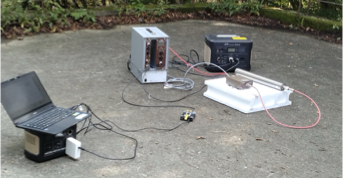
\includegraphics[width=0.95\linewidth]{装置写真.png}\\[0.4em]
{\footnotesize 左：ノート PC・モバイルバッテリー　中：電源回路　右：He-3 比例計数管（測定器）}
{\footnotesize \\実際の占有面積は写真の1/3程度です。}
\end{center}

\end{document}
